%% --------------------------------------------------------------
%%
%% N R  S I M U L A T I O N S
%%
%% --------------------------------------------------------------
\begin{frame}{} %% ---------- title 
\begin{tikzpicture}[overlay,remember picture]
%\uncover<1->{ % <-> |
%    \node (t1) [anchor=center,scale=1,opacity=1] at ([shift={(-0.0cm,-0.2cm)}]current page.center){
%        \parbox{1.1\textwidth}{
%            A prime tool to understand these processes is NR models \\
%            \wisky{} code$^\text{\citep{Radice:2013apa,Radice:2012cu,Radice:2013xpa,Radice:2013hxh,
%                                 Radice:2015nva,Radice:2016dwd,Radice:2018pdn,Radice:2020ids}}$
%            \begin{itemize}
%                \item Eqs. of GR in Z4c formulation via FD method
%                \item Eqs. of GRHD in a conservative form via KT central scheme
%                \item Neutrino radiation transport via Leakage + M0 scheme
%                \item Turbulent viscosity of magnetic origin via GRLES approach
%                \item Microphsyical EOS with finite temperature effects
%            \end{itemize}
%            Overall, $37$ unique simulations targeted to \GW{}, (total of $76$, some $100+$~ms) \\
%    }};
%}
\uncover<1->{ % <-> |
    \node (t1) [anchor=center,scale=1,opacity=1] at ([shift={(-0.0cm,2.9cm)}]current page.center){
        \parbox{1.1\textwidth}{
            \textcolor{blue}{NR models with \wisky{} code}$^\text{\citep{Radice:2013apa,
%                    Radice:2012cu,Radice:2013xpa,Radice:2013hxh,
%                    Radice:2015nva,Radice:2016dwd,Radice:2018pdn,
                    Radice:2020ids}}$. Work with Radice, D., Bernuzzi. S., Perego, A., 
            Breschi, M., Endrizzi, A., Logoteta, D., Prakash, A., Schianchi, F., Zappa, F.

%            \begin{itemize}
%                \item Eqs. of GR in Z4c formulation via FD method
%                \item Eqs. of GRHD in a conservative form via KT central scheme
%                \item Neutrino radiation transport via Leakage + M0 scheme
%                \item Turbulent viscosity of magnetic origin via GRLES approach
%                \item Microphsyical EOS with finite temperature effects
%            \end{itemize}
            Overall, \textcolor{blue}{$37$} $(76)$ \textcolor{blue}{models for \GW{}; some $100+$~ms}. 
            \textbf{ $\{ q, \tilde{\Lambda} \cdots \} \textcolor{blue}{\rightarrow} \{ M_{\rm ej}, \upsilon_{ej} \cdots \}$ }
    }};
}
%\uncover<2->{ % <-> |
%    \node (t1) [anchor=center,scale=1,opacity=1] at ([shift={(-0.0cm,-3.4cm)}]current page.center){
%        \parbox{1.1\textwidth}{
%            \textbf{Goal}: Analyzed ejecta/\nuc{}/EM counterparts \& statistical analysis \\
%            \textbf{Method}: post-processing pipeline \texttt{bns\_ppr\_tools} for ejecta/disk/remnant
%            \begin{itemize}
%            \item Developped post-processing pipeline \texttt{bns\_ppr\_tools}
%            \item \textbf{Goal}: Analyzed for ejecta/\nuc{}/EM counterparts \& statistical analysis
%%            \item Statisitcal analysis alongside other models in literature
%            \end{itemize}
%    }};
%}
\uncover<1->{ % <-> |
    \node (t1) [anchor=center,scale=1,opacity=1] at ([shift={(-2.0cm,1.4cm)}]current page.center){
        \parbox{0.6\textwidth}{
            \small{\textbf{Dynamical Ejecta Properties}}:  \\
    }};
}
\uncover<1->{ % <-> |
    \node (img1) [anchor=center,scale=1,opacity=1] at ([shift={(-3.0cm,-1.5cm)}]current page.center){
        \parbox{0.5\textwidth}{
            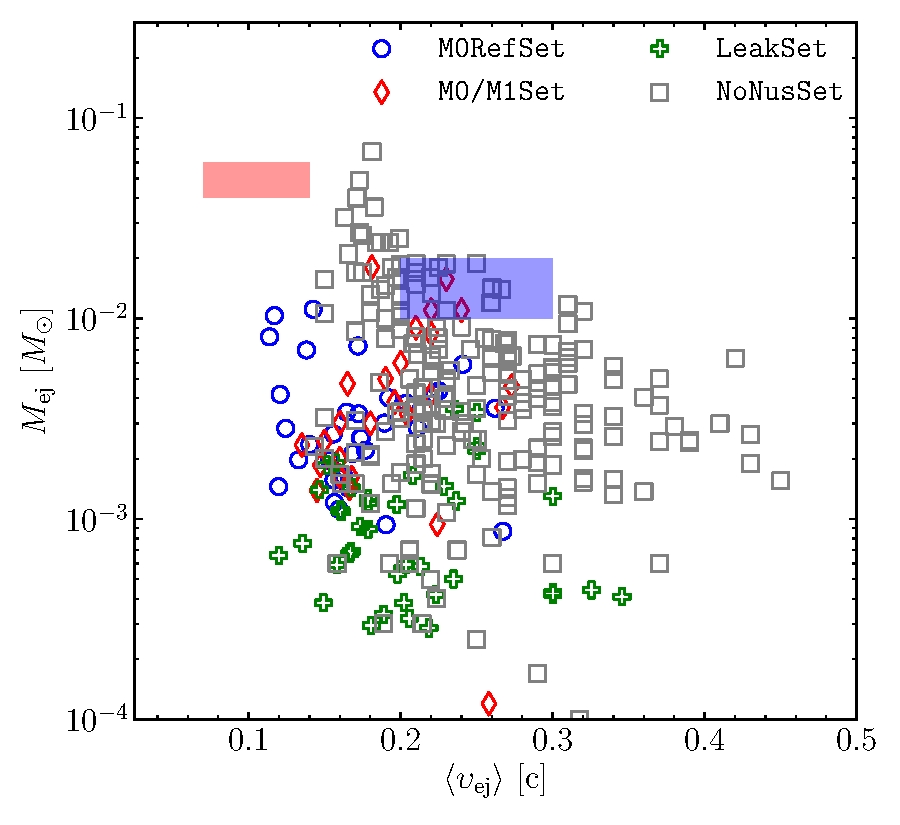
\includegraphics[height=5.4cm]{statistics/ej_mej_vej_groups.pdf} 
            
            \vspace*{-3mm}
            \tiny{ VN+21 \textcolor{gray}{arXiv:2011.11110} } 
            %                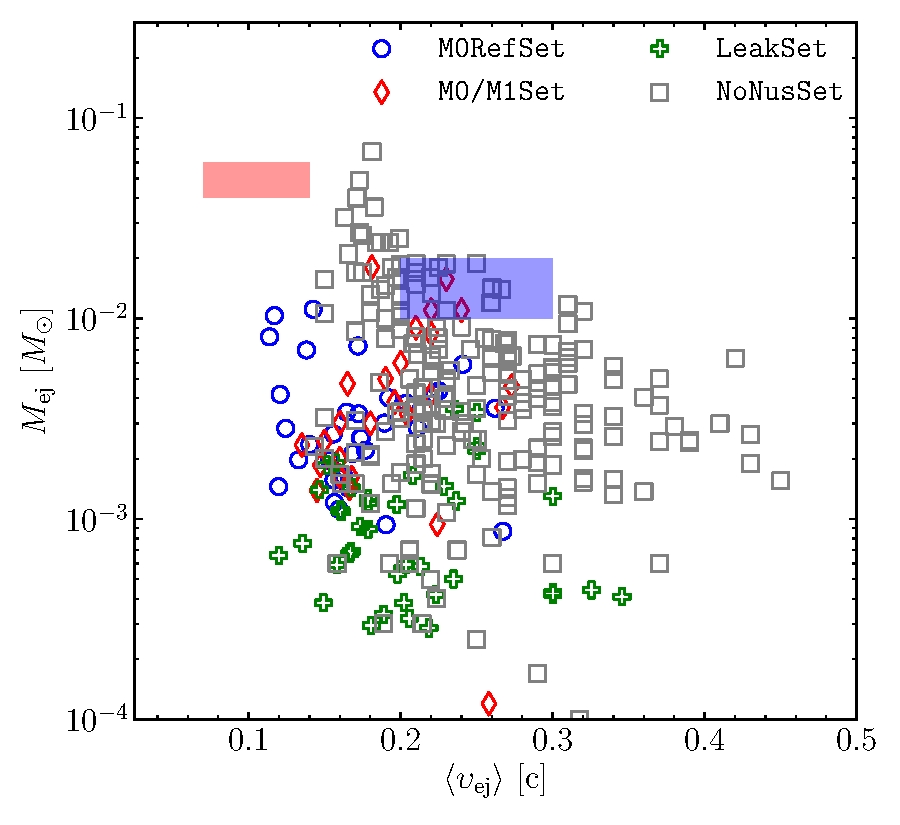
\includegraphics[width=0.32\textwidth]{statistics/ej_mej_vej_groups.pdf}
            %                \includegraphics[width=0.32\textwidth]{statistics/ej_mej_yeej_groups.pdf}
            %                \includegraphics[width=0.32\textwidth]{statistics/ej_vej_yeej_groups.pdf}
            %                \caption{Summary of dynamical ejecta properties used in this work.
            %                    Blue circles represent models of \DSrefset{}, 
            %                    red diamonds stands for models from \DSheatcool{}, 
            %                    green crosses are models from \DScool{}
            %                    and gray squares stand for models from \DSnone{}, 
            %                    %% 
            %                    We show for comparison the two-component fit to AT2017gfo as
            %                    colored patches from \cite{Villar:2017wcc,Siegel:2019mlp}.
            %                    (Adapted from \citet{Nedora:2020qtd})
    }};
}

\uncover<1->{ % <-> |
    \node (t1) [anchor=center,scale=1,opacity=1] at ([shift={(6.0cm,1.4cm)}]current page.center){
        \parbox{0.6\textwidth}{
            \small{\textbf{Spiral arms in disk -- wind origin}}  \\
    }};
}
\uncover<1-1>{ % <-> |
    \node (img1) [anchor=center,scale=1,opacity=1] at ([shift={(5.0cm,-1.4cm)}]current page.center){
        \parbox{0.5\textwidth}{
            \includegraphics[height=5.2cm]{raycasting_smooth_cropped.pdf}
            
            %\hspace*{2.8mm}Spiral arms within the disk
            \vspace*{-0mm}
            \tiny{ VN+19 \textcolor{gray}{arXiv:1907.04872} } 
    }};
}
\end{tikzpicture}
\end{frame}